\documentclass[svgnames,11pt]{beamer}
\input{/home/tof/Documents/Cozy/latex-include/preambule_commun.tex}
\input{/home/tof/Documents/Cozy/latex-include/preambule_beamer.tex}
%\usepackage{pgfpages} \setbeameroption{show notes on second screen=left}
\author[]{Christophe Viroulaud}
\title{Géocube mesures}
\date{\framebox{\textbf{Donn 02}}}
%\logo{}
\institute{Seconde - SNT}

\begin{document}
\begin{frame}
    \titlepage
\end{frame}
\begin{frame}
    \frametitle{}
    \begin{center}
        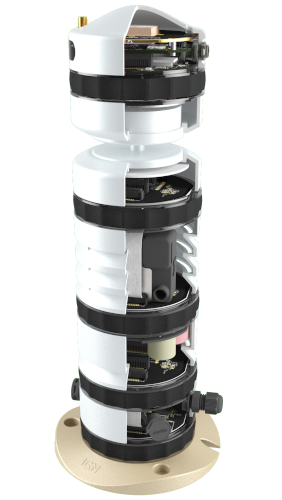
\includegraphics[width=3cm]{ressources/geocube-interne.png}
        \captionof{figure}{Le Géocube effectue de nombreuses mesures par jour.
        }
    \end{center}

\end{frame}
\begin{frame}
    \frametitle{}

    \begin{framed}\centering
        Comment manipuler de grandes quantités de données?
    \end{framed}

\end{frame}
\section{Stocker des données}
\begin{frame}
    \frametitle{Stocker des données}
    Les données fournies par le Géocube sont stockées dans un fichier \emph{csv}.
    \begin{center}
        nom,prenom,naissance\\
        Dupont,John,2006-12-09\\
        Durant,James,2008-06-10
    \end{center}
    \begin{aretenir}[]
        Un fichier \textbf{csv (Comma Separated Values)} stocke les données sous forme de tableau. Une donnée est caractérisée par ses \textbf{descripteurs}. \\
        Chaque valeur est séparée par un caractère spécial: une virgule, un point-virgule, une tabulation\dots
    \end{aretenir}

\end{frame}
\begin{frame}
    \frametitle{}

    \begin{activite}
        \begin{enumerate}
            \item Se rendre sur le site \url{https://geobs.fr/cartograph/}.
            \item À l'aide de l'onglet \textbf{\texttt{recherche}} trouver le géocube \textbf{Albert de Mun}.
            \item Dans quelle ville se trouve cet appareil? Où est-il situé par rapport à Paris?
            \item Cliquer sur \textbf{\texttt{Ajouter}} puis \textbf{\texttt{Voir les données}}.
        \end{enumerate}
    \end{activite}

\end{frame}
\begin{frame}
    \frametitle{Avant de regarder la correction}
    \begin{center}
        \centering
        \includegraphics[width=3cm]{/home/tof/Documents/Cozy/latex-include/stop.png}
    \end{center}
    {\Large
    \begin{itemize}
        \item Prendre le temps de réfléchir,
        \item Analyser les messages d'erreur,
        \item Demander au professeur.
    \end{itemize}
    }
\end{frame}
\begin{frame}
    \frametitle{Correction}

    Le géocube Albert de Mun se trouve à Nogent-sur-Marne au sud-est de Paris.

\end{frame}
\begin{frame}
    \frametitle{}

    \begin{activite}
        \begin{enumerate}
            \item Sélectionner la journée du samedi 4 décembre 2021.
            \item Sélectionner la \textbf{Pression} et la \textbf{Température} (attention il faut sélectionner la température située en dessous de \textbf{Humidité} et non la première).
            \item Appliquer les modifications.
            \item Télécharger les fichiers \textbf{\texttt{csv}} pour chaque donnée.
        \end{enumerate}
    \end{activite}

\end{frame}
\begin{frame}
    \frametitle{Avant de regarder la correction}
\begin{center}
    \centering
    \includegraphics[width=3cm]{/home/tof/Documents/Cozy/latex-include/stop.png}
    \end{center}
{\Large
    \begin{itemize}
        \item Prendre le temps de réfléchir,
        \item Analyser les messages d'erreur,
        \item Demander au professeur.
    \end{itemize}
}
\end{frame}
\begin{frame}
    \frametitle{Correction}

    \begin{center}
        En cas de problème télécharger le dossier compressé
        \href{https://cviroulaud.github.io/seconde/donnees/geocube-mesures/scripts/donnees-4decembre.zip}{en cliquant ici}.
    \end{center}

\end{frame}
\begin{frame}
    \frametitle{}

\begin{activite}
\begin{enumerate}
    \item Ouvrir un nouveau classeur LibreOffice et l'enregistrer sous le nom \textbf{\texttt{albert-4dec-votrenom}}.
    \item Ouvrir le fichier \textbf{\texttt{Pression.csv}}. Quelles informations contient-il?
    \item Quelle est la fréquence des enregistrements?
    \item Copier la seconde colonne et la coller dans le classeur \textbf{\texttt{albert-4dec\dots}}
    \item Faire de même avec le fichier \textbf{\texttt{Temprature.csv}}
\end{enumerate}
\end{activite}
\end{frame}
\begin{frame}
    \frametitle{Avant de regarder la correction}
\begin{center}
    \centering
    \includegraphics[width=3cm]{/home/tof/Documents/Cozy/latex-include/stop.png}
    \end{center}
{\Large
    \begin{itemize}
        \item Prendre le temps de réfléchir,
        \item Analyser les messages d'erreur,
        \item Demander au professeur.
    \end{itemize}
}
\end{frame}
\begin{frame}
    \frametitle{Correction}
    Le fichier de pression contient la date et la pression pour chaque mesure. Un enregistrement est effectué toutes les 10 minutes.

    

\end{frame}
\section{Manipuler des données}
\begin{frame}
    \frametitle{Manipuler les données}

Le logiciel ne reconnaît pas automatiquement les données comme des nombres. Il faut adapter le contenu des cellules en transformant les points en virgules.
\begin{activite}
\begin{enumerate}
    \item Sélectionner l'ensemble des données.
    \item Dans le menu \textbf{\texttt{Édition}}, choisir \textbf{\texttt{Rechercher \& remplacer}}.
    \item Remplacer \underline{tous} les points par des virgules.
\end{enumerate}
\end{activite} 

\end{frame}
\begin{frame}
    \frametitle{}

    \begin{activite}
    \begin{enumerate}
        \item Sélectionner l'ensemble des données.
        \item Choisir l'icône \textbf{Insérer un diagramme}
        \begin{center}
        \centering
        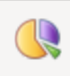
\includegraphics[width=1cm]{ressources/diag.png}
        \captionof{figure}{L'image peut varier.}
        \label{IMG}
        \end{center}
        \item Choisir le modèle \textbf{Dispersion} puis cliquer sur \textbf{Terminer}.
        \item Que représente le nuage de points obtenus?
    \end{enumerate}
    \end{activite}

\end{frame}
\begin{frame}
    \frametitle{Avant de regarder la correction}
\begin{center}
    \centering
    \includegraphics[width=3cm]{/home/tof/Documents/Cozy/latex-include/stop.png}
    \end{center}
{\Large
    \begin{itemize}
        \item Prendre le temps de réfléchir,
        \item Analyser les messages d'erreur,
        \item Demander au professeur.
    \end{itemize}
}
\end{frame}
\begin{frame}
    \frametitle{Correction}

    \begin{center}
    \centering
    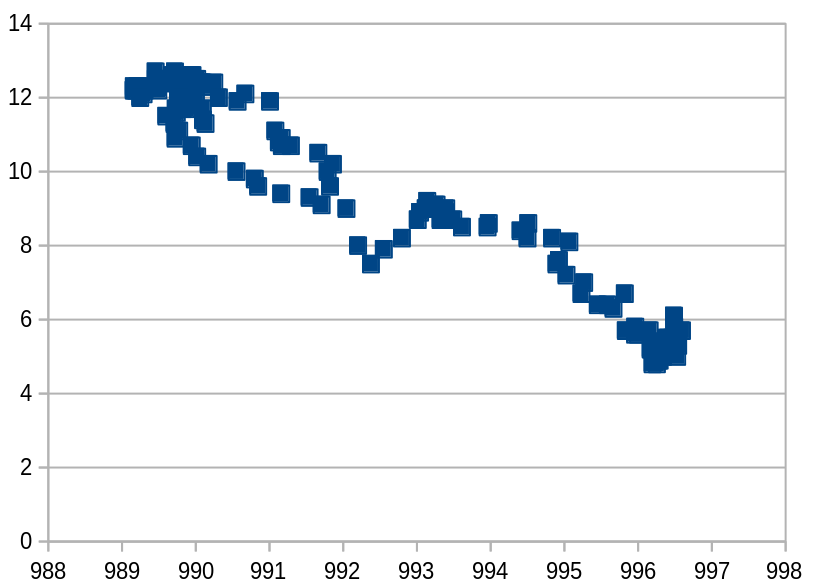
\includegraphics[width=10cm]{ressources/nuage.png}
    \captionof{figure}{\centering Température en fonction de la pression}
    \label{IMG}
    \end{center}

\end{frame}
\section{Interpréter des données}   
\begin{frame}
    \frametitle{Interpréter des données}

\begin{aretenir}[]
    Une représentation graphique peut montrer une tendance. On parle de \textbf{corrélation} entre deux grandeurs quand le nuage de points obtenus semble suivre une courbe ou une droite.
\end{aretenir}
\vspace{1cm}
\begin{tabular}{cc}
    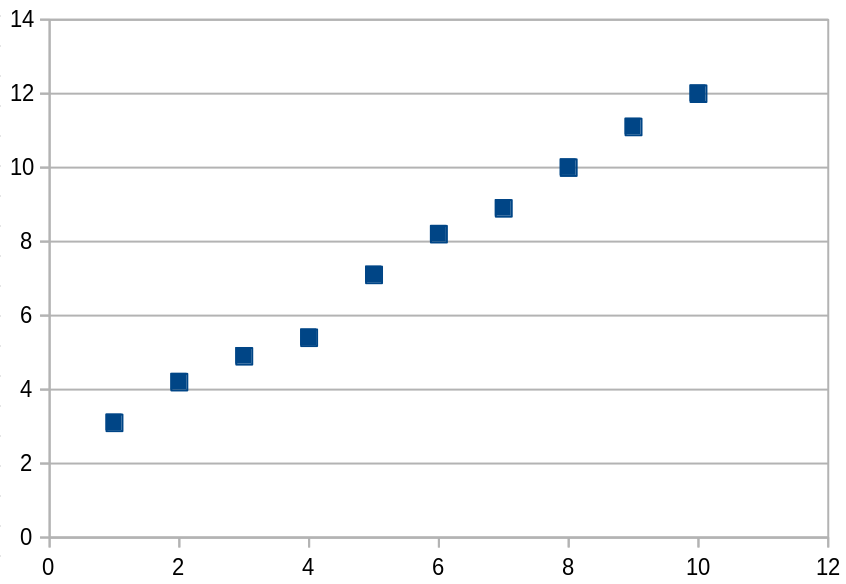
\includegraphics[width=4.5cm]{ressources/correlation.png}
    &
    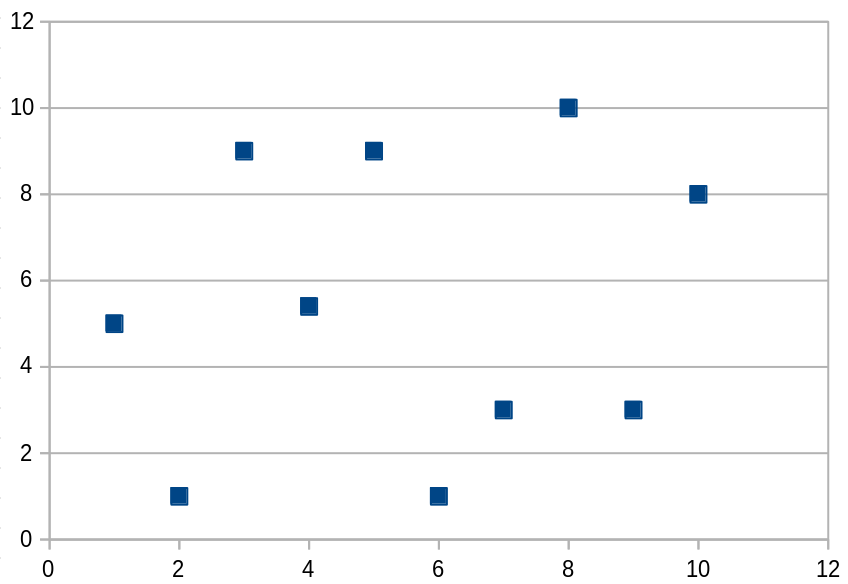
\includegraphics[width=4.5cm]{ressources/pas-cor.png}\\
    corrélation&pas de corrélation
\end{tabular}   

\end{frame}
\begin{frame}
    \frametitle{}

    \begin{aretenir}[]
    On peut calculer une \textbf{courbe de tendance} ou courbe de régression. On peut l'assimiler à la courbe (ou la droite) \emph{moyenne} du nuage de points.
    \end{aretenir}

\end{frame}
\begin{frame}
    \frametitle{}

    \begin{activite}
    \begin{enumerate}
        \item la température et la pression semblent-elles être en corrélation?
        \item Double-cliquer sur la représentation graphique puis cliquer sur un des points pour tous sélectionner le jeu de données.
        \item Dans le menu \textbf{\texttt{Insertion}}, choisir \textbf{courbe de tendance}.
        \item Garder le réglage \textbf{\texttt{linéaire}} et valider.
        \item Que peut-on dire à propos de la température quand la pression augmente?
    \end{enumerate}
    \end{activite}

\end{frame}
\begin{frame}
    \frametitle{Avant de regarder la correction}
\begin{center}
    \centering
    \includegraphics[width=3cm]{/home/tof/Documents/Cozy/latex-include/stop.png}
    \end{center}
{\Large
    \begin{itemize}
        \item Prendre le temps de réfléchir,
        \item Analyser les messages d'erreur,
        \item Demander au professeur.
    \end{itemize}
}
\end{frame}
\begin{frame}
    \frametitle{Correction}

    \begin{center}
    \centering
    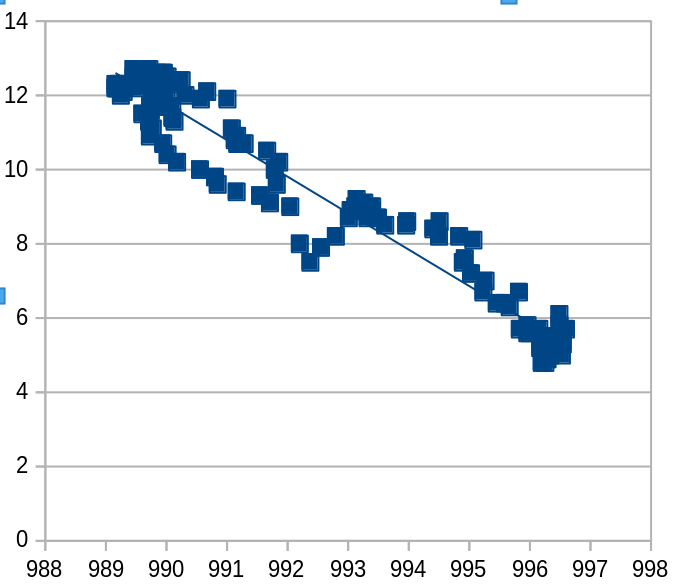
\includegraphics[width=7.5cm]{ressources/temp-press.png}
    \captionof{figure}{Corrélation entre la température et la pression}
    \label{IMG}
    \end{center}
Quand la pression atmosphérique augmente, la température diminue.
\end{frame}
\begin{frame}
    \frametitle{}

    \begin{aretenir}[]
    Corrélation ne signifie pas \underline{obligatoirement} causalité: deux grandeurs peuvent varier ensembles mais ne pas être liées.
    \end{aretenir}
Exemple:
\begin{itemize}
    \item En été les vendeurs de glace vendent beaucoup plus de glaces qu'en hiver.
    \item En été il y a beaucoup plus de cas de noyades qu'en hiver.
\end{itemize}
Les données sont en corrélation, mais on ne peut pas mettre en cause les glaciers dans les cas de noyade.
\end{frame}
\end{document}